%-------------------------
% Resume in Latex
% Author : Aiden
%------------------------

\documentclass[letterpaper,11pt]{article}

\usepackage{latexsym}
\usepackage[empty]{fullpage}
\usepackage{titlesec}
\usepackage{marvosym}
\usepackage[usenames,dvipsnames]{color}
\usepackage{verbatim}
\usepackage{enumitem}
\usepackage[hidelinks]{hyperref}
\usepackage{fancyhdr}
\usepackage[english]{babel}
\usepackage{tabularx}
\usepackage{xcolor}
\usepackage{fontawesome5}
\usepackage{graphicx}

\input{glyphtounicode}

% -------------------- FONT OPTIONS --------------------
% sans-serif
% \usepackage[sfdefault]{roboto}
% \usepackage[sfdefault]{noto-sans}
% serif
% \usepackage{charter}

\pagestyle{fancy}
\fancyhf{} % clear all header and footer fields
\fancyfoot{}
\renewcommand{\headrulewidth}{0pt}
\renewcommand{\footrulewidth}{0pt}

% Adjust margins
\addtolength{\oddsidemargin}{-0.5in}
\addtolength{\evensidemargin}{-0.5in}
\addtolength{\textwidth}{1in}
\addtolength{\topmargin}{-1in} % Default was -.5in
\addtolength{\textheight}{1.0in}

\urlstyle{same}

\raggedbottom
\raggedright
\setlength{\tabcolsep}{0in}

% Section formatting
\titleformat{\section}{
  \vspace{-5pt}\scshape\raggedright\large
}{}{0em}{}[\color{black}\titlerule \vspace{-5pt}]

% Subsection formatting
\titleformat{\subsection}{
  \vspace{-4pt}\scshape\raggedright\large
}{\hspace{-.15in}}{0em}{}[\color{black}\vspace{-8pt}]

% Ensure that generate pdf is machine readable/ATS parsable
\pdfgentounicode=1

% -------------------- CUSTOM COMMANDS --------------------
\newcommand{\resumeItem}[1]{
  \item\small{
    {#1 \vspace{-2pt}}
  }
}

\newcommand{\resumeSubheading}[4]{
  \vspace{-2pt}\item
    \begin{tabular*}{0.97\textwidth}[t]{l@{\extracolsep{\fill}}r}
      \textbf{#1} & #2 \\
      \textit{\small#3} & \textit{\small #4} \\
    \end{tabular*}\vspace{-7pt}
}

\newcommand{\resumeSubSubheading}[2]{
    \item
    \begin{tabular*}{0.97\textwidth}{l@{\extracolsep{\fill}}r}
      \textit{\small#1} & \textit{\small #2} \\
    \end{tabular*}\vspace{-7pt}
}

\newcommand{\resumeProjectHeading}[2]{
    \item
    \begin{tabular*}{0.97\textwidth}{l@{\extracolsep{\fill}}r}
      \small#1 & #2 \\
    \end{tabular*}\vspace{-7pt}
}

\newcommand{\resumeSubItem}[1]{\resumeItem{#1}\vspace{-4pt}}
\newcommand{\resumeSubHeadingListStart}{\begin{itemize}[leftmargin=0.15in, label={}]}
\newcommand{\resumeSubHeadingListEnd}{\end{itemize}}
\newcommand{\resumeItemListStart}{\begin{itemize}}
\newcommand{\resumeItemListEnd}{\end{itemize}\vspace{-5pt}}

\renewcommand\labelitemii{$\vcenter{\hbox{\tiny$\bullet$}}$}

\setlength{\footskip}{4.08003pt}

% -------------------- START OF DOCUMENT --------------------
\begin{document}

% -------------------- HEADING--------------------
\begin{flushright}
  % \vspace{-4pt}
  \color{gray}
  \item
  Last Updated on March 19th, 2025
\end{flushright}

\vspace{-5pt}

\raisebox{-.7\totalheight}[0pt][.5\totalheight]{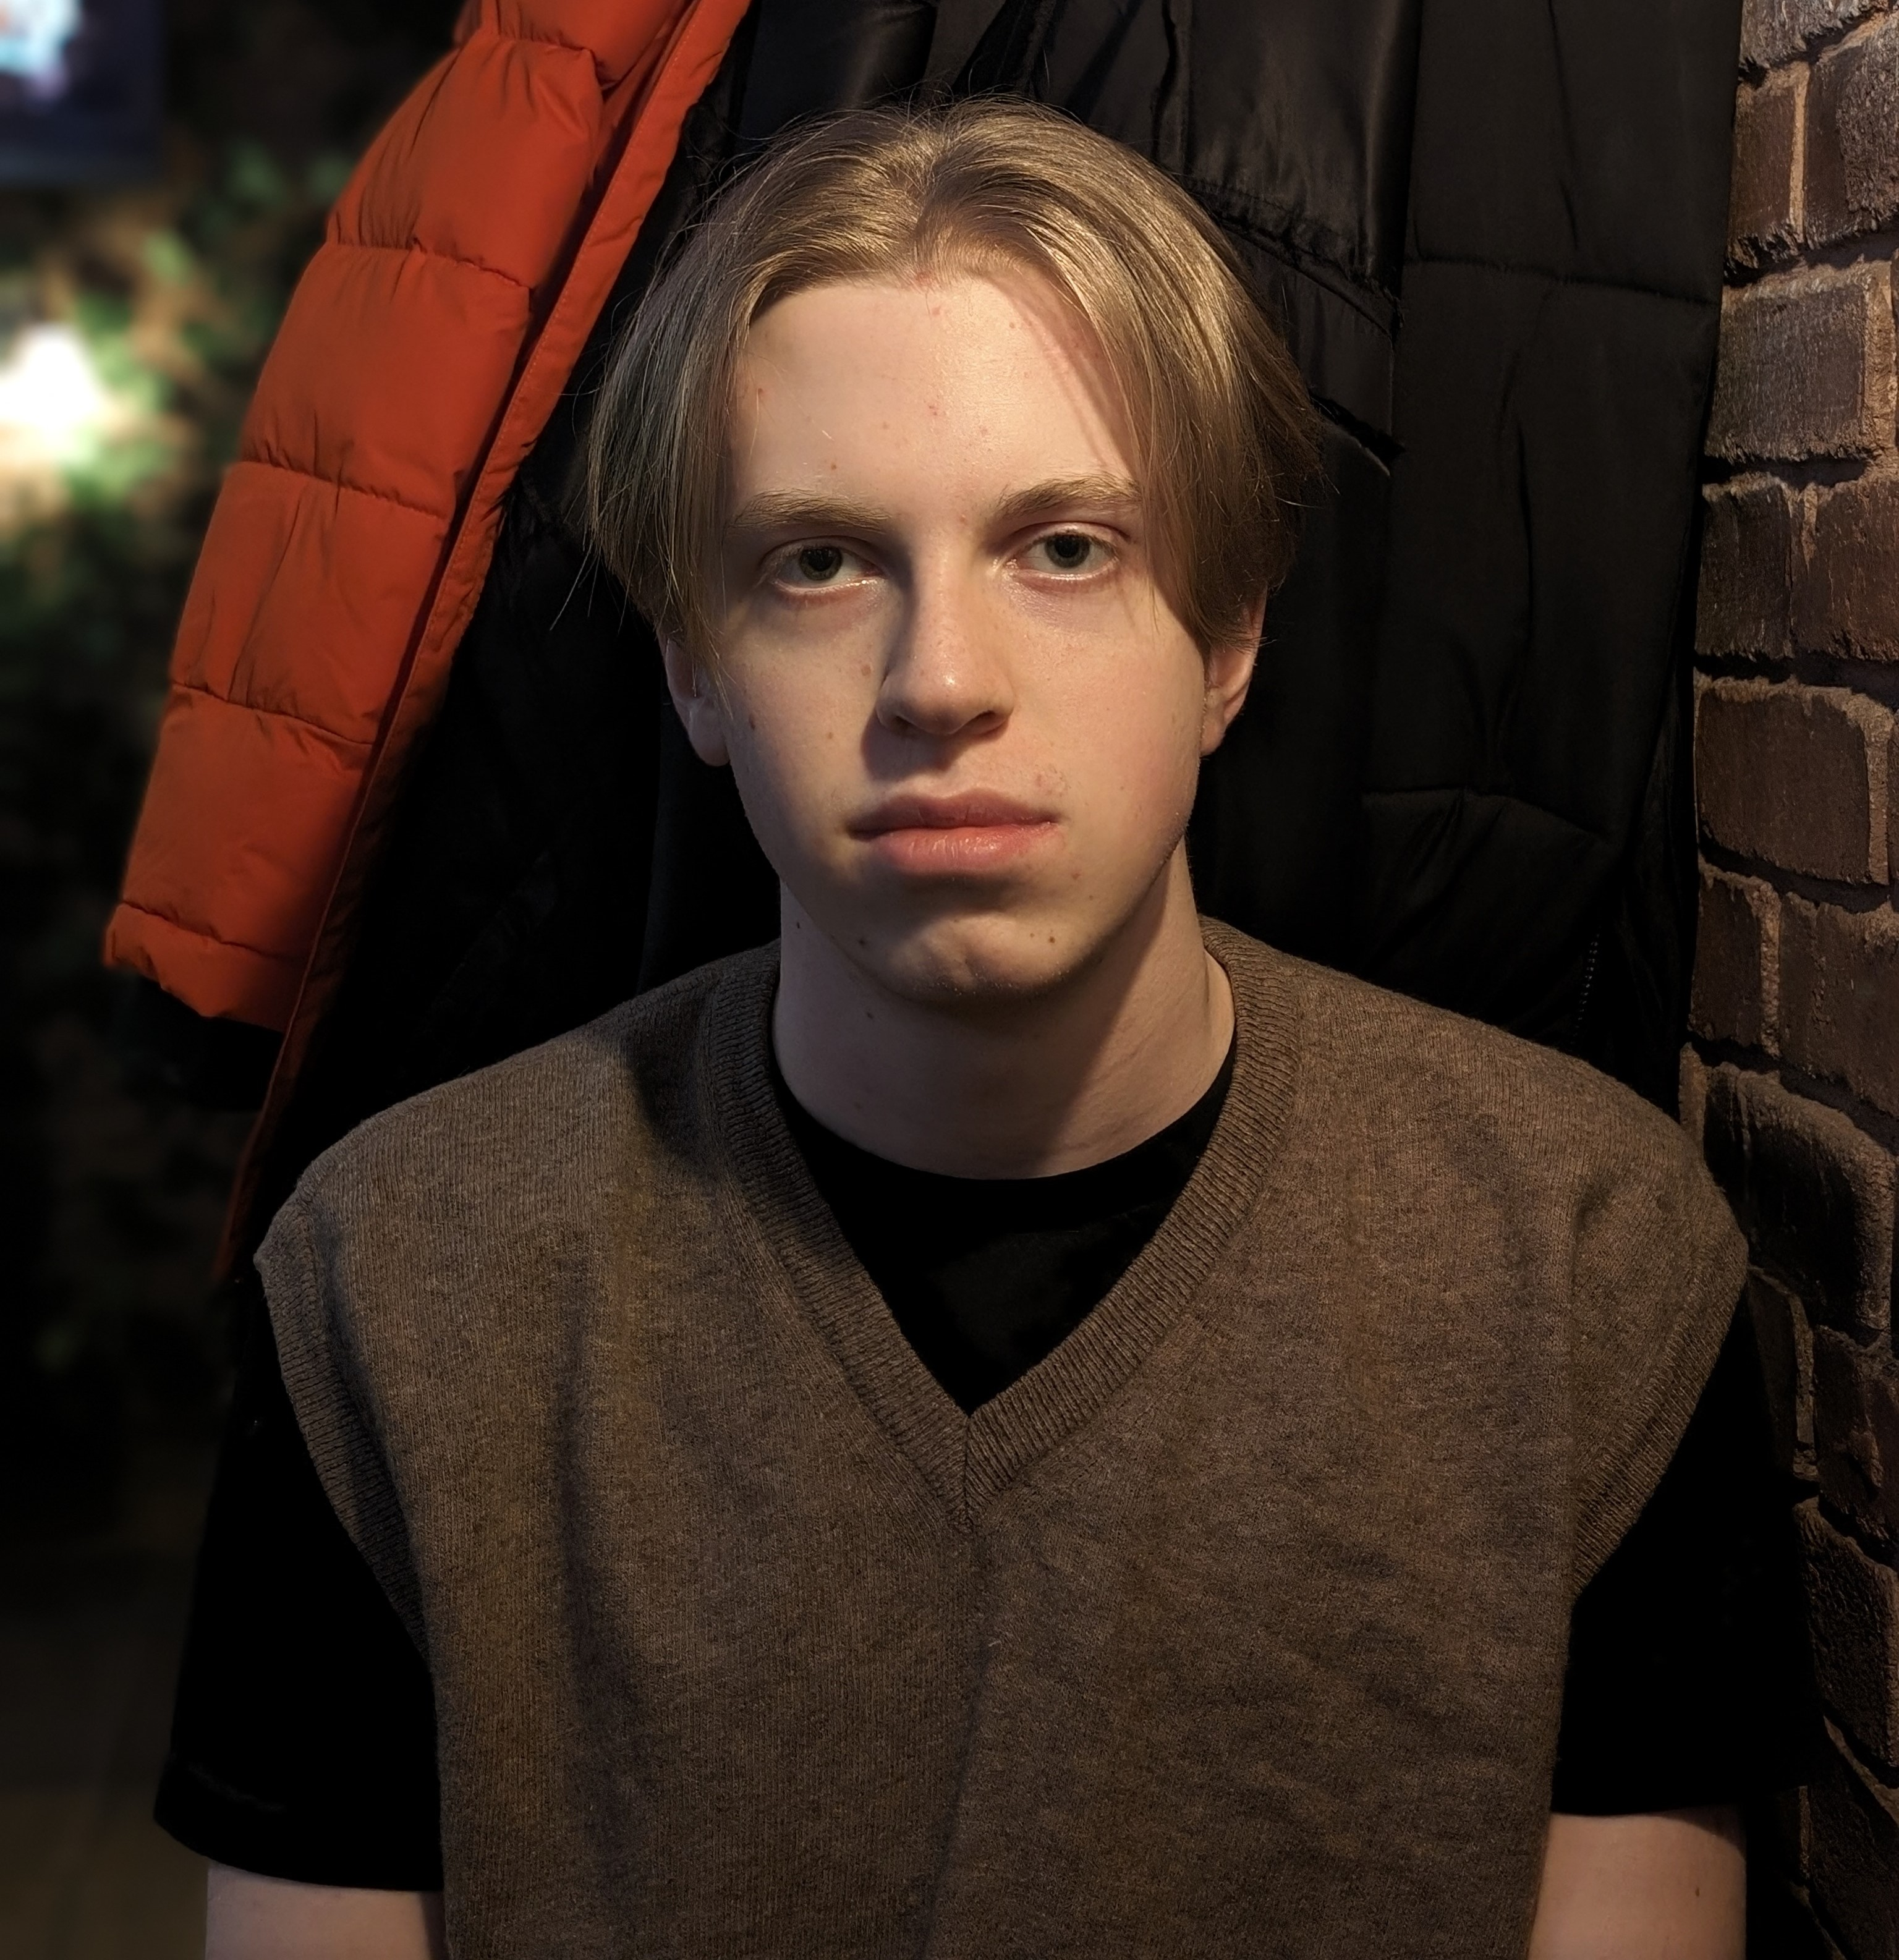
\includegraphics[width=3cm,height=3.5cm]{img/profile.jpg}}

\begin{center}
    \textbf{\Huge \scshape Aiden Munro} \\ \vspace{8pt}
    \small 
    \faIcon{github}
    \href{https://github.com/aidenfmunro}{\underline{github.com/aidenfmunro}} $  $
    \faIcon{envelope}
    \href{mailto:manro.e@phystech.edu}{\underline{manro.e@phystech.edu}} $ $
    \faIcon{mobile}
    \underline{+7 915 298 11 30} 
    \faIcon{home}
    Moscow, Russia
\end{center}

% -------------------- EDUCATION --------------------
\section{Education}
  \resumeSubHeadingListStart
  
    \resumeSubheading
      {MIPT}{2023 - 2027}
      {Department of Radio Engineering and Cybernetics}{Overall GPA: 8.0/10, Programming GPA: 7.5/10}

    \vspace{-10pt}

    \subsection{Coursework}
      \textbf{Courses:} C/C++ Programming, Assembly, Discrete Math, Linear Algebra, Calculus, Physics, Probability \& Statistics \\
      \textbf{Awards:} Russian National Olympiad in Mathematics Region Prize Winner (4x), MIPT Olympiad in Mathematics Prize Winner, MSU Olympiad in Physics Prize Winner, BMSTU Olympiad in Physics Prize Winner, Physics EGE 100 points.

  \resumeSubHeadingListEnd

% -------------------- SKILLS --------------------
\section{Skills}
 \begin{itemize}[leftmargin=0.15in, label={}]
    \small{\item{
    
     \textbf{Languages}{: C/C++, NASM, Python, \LaTeX, DOT} \\
     
     \textbf{Tools}{: Git/GitHub, Linux, VS Code, Make, GDB, Kcachegrind, perf, hotspot, IDA, SDL, SFML}
     
     % \textbf{Frameworks}{: React, Node.js, Flask, JUnit, WordPress, Material-UI, FastAPI} \\
     
     % \textbf{Libraries}{: pandas, NumPy, Matplotlib}
     
    }}
 \end{itemize}

% -------------------- PROJECTS --------------------
\section{Projects}
    \resumeSubHeadingListStart

        \resumeProjectHeading
        {\textbf{CPU} {\color{blue}\href{https://github.com/aidenfmunro/CPU}{[GitHub]}} $|$ \footnotesize\emph{C/C++, SDL}}{Oct. 2023}
        \resumeItemListStart
            \resumeItem{An implementation of my own simplified virtual machine that simulates the work of a single processor unit. The project is split into three seperate programs: an assembler, a disassembler, and the machine itself. The assembly language is made by me. As an additional task the ASCII represantation of the famous Bad Apple video was ran on my CPU using it's RAM as video memory.}
          \resumeItemListEnd
    
        \resumeProjectHeading
        {\textbf{Cache-friendly doubly linked list} {\color{blue}\href{https://github.com/aidenfmunro/LinkedList}{[GitHub]}} $|$ \footnotesize\emph{C/C++, DOT}}{Nov. 2023}
        \resumeItemListStart
            \resumeItem{A cache friendly doubly linked list is a data structure based on nodes.
            In a cache friendly doubly linked list the nodes are arranged contiguously in memory, minimizing the number of cache misses when accessing consecutive nodes. Also the canonical version of the linked list was made. For better debugging experience DOT language was used to dump images of the current state of the linked list.}
          \resumeItemListEnd
          
        \resumeProjectHeading
        {\textbf{Programming language}  {\color{blue}\href{https://github.com/aidenfmunro/Scotlang}{[GitHub]}} $|$ \footnotesize\emph{C/C++, DOT}}{Feb. 2024}
        \resumeItemListStart
            \resumeItem{My Scottish programming language. It consists of a Tokenizer, Parser \& Compiler. The Tokenizer reads the source file and creates token. The Parser uses recursive descent algorithm to build an Abstract Syntax Tree. The Compiler then analyzes the AST and translates it into instructions of my assembly language.}
        \resumeItemListEnd

        \resumeProjectHeading
        {\textbf{Mandelbrot Set}  {\color{blue}\href{https://github.com/aidenfmunro/MandelbrotSet}{[GitHub]}} $|$ \footnotesize\emph{C/C++, SFML}}{Mar. 2024}
        \resumeItemListStart
            \resumeItem{Visualization of the Mandelbrot fractal. SIMD instructions were used to optimize image processing.}
        \resumeItemListEnd

        \resumeProjectHeading
        {\textbf{Hash Table optimization}  {\color{blue}\href{https://github.com/aidenfmunro/HashTable}{[GitHub]}} $|$ \footnotesize\emph{C/C++, Python, NASM, GCC inline assembly, perf, hotspot}}{Apr. 2024}
        \resumeItemListStart
            \resumeItem{Hash Table data structure implementation using my linked list. This project is split into 2 parts: Hash functions analysis \& Hash Table optimization. Histograms of different hash distributions were made using matplotlib in python. Further optimizations were made using GCC inline assembly, assembly written function \& intrinsics that were analyzed using hotspot \& perf.}
        \resumeItemListEnd

        \resumeProjectHeading
        {\textbf{Linux Course}  {\color{blue}\href{https://github.com/aidenfmunro/Linux-Course}{[GitHub]}} $|$ \footnotesize\emph{C, Python}}{Sep-Nov. 2024}
        \resumeItemListStart
            \resumeItem{UNIX-Like OS programming in Userspace (IPC, multithreading, TCP/IP, daemons, etc.)}
        \resumeItemListEnd

        \newpage
        
        \resumeProjectHeading
        {\textbf{ParaCL}  {\color{blue}\href{https://github.com/aidenfmunro/ParaCL}{[GitHub]}} $|$ \footnotesize\emph{C++, Flex, Bison}}{WIP 2025}
        \resumeItemListStart
            \resumeItem{Interpreted C-like Programming Language made with using tools such as Flex and Bison. Co-developing the frontend and AST.}
        \resumeItemListEnd  
    \resumeSubHeadingListEnd

\vspace{20pt}

% -------------------- Soft skills --------------------
\section{Soft skills}
    \begin{itemize}
        \item Adaptability, self motivation, attention to detail, verbal communication, emotional intelligence, work ethic, resilience, humility. 
    \end{itemize}


\end{document}
